\documentclass{article}
\usepackage{a4wide}
\usepackage[english]{babel}
\usepackage{amsmath}
\usepackage{amssymb}
\usepackage{dsfont}
%\usepackage[dvips]{epsfig}
%\usepackage{graphicx}
\usepackage{fancyhdr}
\usepackage{listings}
\usepackage{nomencl}
\usepackage[pdftex]{graphicx}

\pagestyle{fancy}
\lhead{\footnotesize \parbox{11cm}{A.J. H\"ormer, E. Vontobel, A. Novacek}}
\rhead{\footnotesize {Plexos Project}}
\chead{\footnotesize {TET4135}}

\title{Report Plexos Project}
\author{Andreas Johann H\"ormer, Eva Vontobel, Adam Novacek}
\date{\today}

\begin{document}
\thispagestyle{empty}
\maketitle
\thispagestyle{empty}
%\\[5cm]
\begin{center}
TET4135 Energiplanlegging\\[3cm]
Lab group:
\begin{itemize}
\item Andreas Johann H\"ormer
\item Eva Vontobel
\item Adam Novacek\\[3cm]
\end{itemize}
Report delivered: \\[6cm]
FACULTY OF INFORMATION TECHNOLOGY, MATHEMATICS AND ELECTRICAL ENGINEERING\\
NORWEGIAN UNIVERSITY OF SCIENCE AND TECHNOLOGY
\end{center}
\thispagestyle{empty}
\newpage
\tableofcontents
\thispagestyle{empty}
\newpage
\section*{Abstract}
\thispagestyle{empty}

\newpage
\setcounter{page}{1}
\section{Introduction}

\section{Theory}
\subsection{Methods in present work}
\subsection{intermittent resource handling}
\subsection{reservoir hydro handling}
\subsection{region exchange}
\subsubsection{Advantages}
\subsubsection{Disadvantages}
\subsection{investment initiatives for renewable sources}
\begin{itemize}
\item investment support\\
One time financial support to cover part of the investment costs.  The support is large enough to make the investment profitable. Some differences can be used for fine tuning, e.g. more support for wind power in areas with less wind.
\begin{itemize}
\item advantages
\begin{itemize}
\item possibility of finetuning
\end{itemize}
\item disadvantages
\begin{itemize}
\item requires much capital at beginning
\item no incentive to roduce
\item limited security for investor
\item in case of fine tuning: much administration
\end{itemize}
\end{itemize}
\item tendering\\
Auction for a certain amount of capacity which shall be installed. Won by the offers requiring the lowest support. This initiative is also done as investment support, but with a tendering procedure. Providers are asked for support bids, the cheapest one gets the support.
\begin{itemize}
\item advantages
\begin{itemize}
\item competition between suppliers, therefore lower costs than investment support
\end{itemize}
\item disadvantages
\begin{itemize}
\item same as investment support, but
\item less predictability
\item prone to corruption
\end{itemize}
\end{itemize}
\item feed-in tariff\\
A fixed price for feeded kWh is payed for a predefined period.
\begin{itemize}
\item advantages
\begin{itemize}
\item promotion of mid-term and long-term technologies
\item investment security for producer
\end{itemize}
\item disadvantages
\begin{itemize}
\item possible risk of technology overfunding
\end{itemize}
\end{itemize}
\item premium\\
Like feed-in tariff, but instead of a fixed price an additional amount per kWh is paid to the producer.
\begin{itemize}
\item advantages
\begin{itemize}
\item market based
\end{itemize}
\item disadvantages
\begin{itemize}
\item less certainty than feed-in tariff
\end{itemize}
\end{itemize}
\item green certificates
\end{itemize}

\section{Analysis}
\subsection{MT Schedule}
\subsubsection{normal inflow scenario}
\paragraph{optimal generation dispatch\\}
\begin{figure}[htbp]
\begin{center}
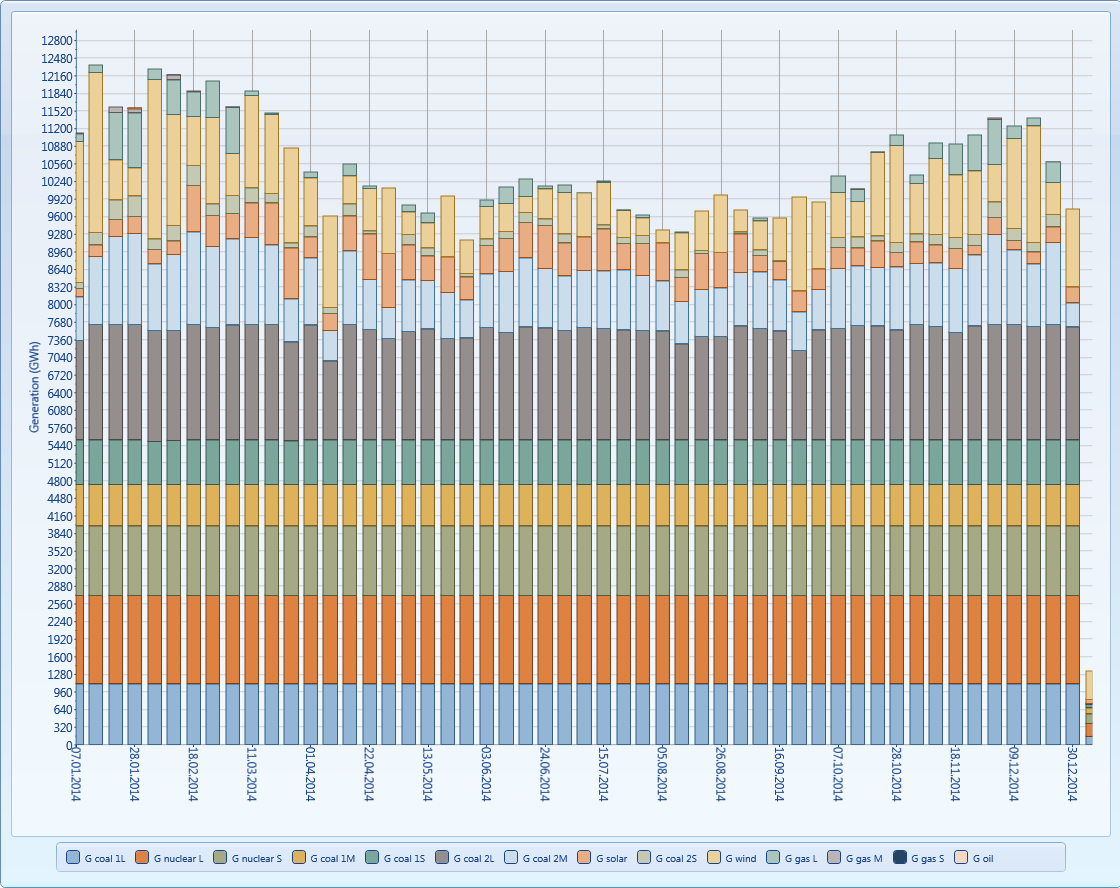
\includegraphics[width=14cm,keepaspectratio=true]{figures/MTgenerationG}
\caption{Optimal generation dispatch for Germany 2014 with normal inflow}
\label{fig:MTgenerationGnormal}
\end{center}
\end{figure}
\begin{figure}[htbp]
\begin{center}
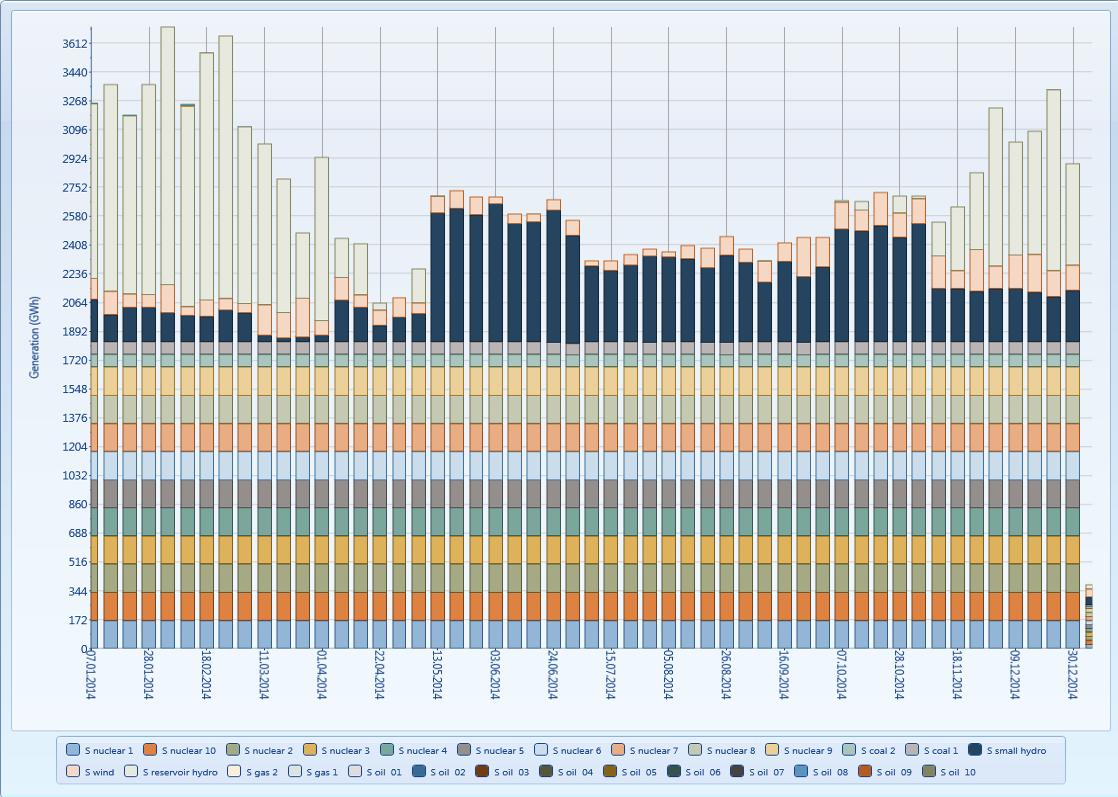
\includegraphics[width=14cm,keepaspectratio=true]{figures/MTgenerationS}
\caption{Optimal generation dispatch for Sweden 2014 with normal inflow}
\label{fig:MTgenerationSnormal}
\end{center}
\end{figure}
\begin{figure}[htbp]
\begin{center}
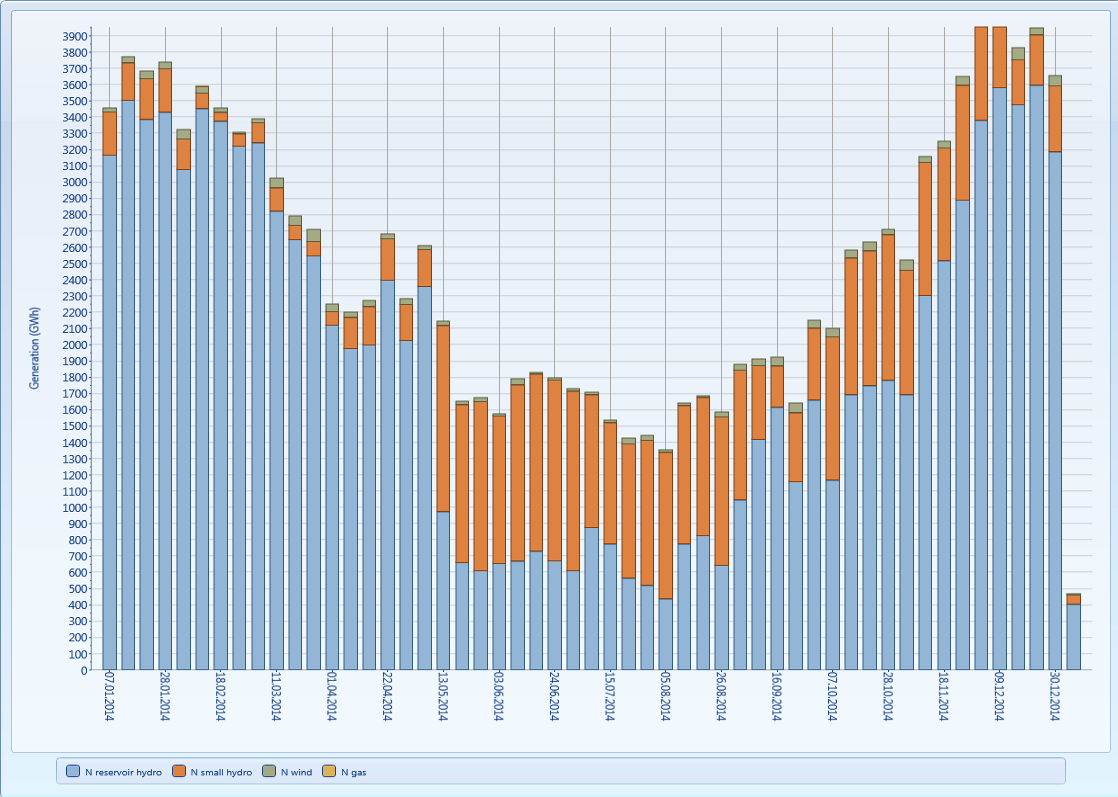
\includegraphics[width=14cm,keepaspectratio=true]{figures/MTgenerationN}
\caption{Optimal generation dispatch for Norway 2014 with normal inflow}
\label{fig:MTgenerationNnormal}
\end{center}
\end{figure}
\paragraph{transmission\\}
\paragraph{emission\\}
\paragraph{price\\}
\subsubsection{high inflow scenario}
\subsubsection{low inflow scenario}
\subsection{Expansion planning}
\newpage
\section{Conclusion}


\end{document}
